\documentclass[14pt,fleqn]{extarticle}
\usepackage[T2A,T1]{fontenc}
\usepackage[utf8]{inputenc}
\usepackage[russian]{babel}
\usepackage{amsmath}
\usepackage{graphicx}
\usepackage{tabularx}
\usepackage{boldline}
\usepackage{makecell}
\usepackage{arydshln}
\usepackage{mathtools}
\usepackage{centernot}
\usepackage{enumitem}
\usepackage{nccmath}
\usepackage{amssymb}
\usepackage[a4paper, total={6.5in, 9.5in}]{geometry}

\graphicspath{ {./images/} }
\setlength{\mathindent}{0pt}
\setlength\parindent{0pt}

\def\at{
	\left.
	\vphantom{\int}
	\right|
}


\begin{document}
	\begin{titlepage}
		
\includegraphics[scale=0.12]{logo}
		\begin{center}
			\textbf{МИНОБРНАУКИ РОССИИ}\\
			\vspace{0.2cm}
			\textbf{Федеральное государственное бюджетное образовательное учреждение высшего образования}\\
			\textbf{<<САНКТ-ПЕТЕРБУРГСКИЙ ГОСУДАРСТВЕННЫЙ ЭКОНОМИЧЕСКИЙ УНИВЕРСИТЕТ>>}\\
			\vspace{0.6cm}
			Факультет информатики и прикладной математики\\
			Кафедра прикладной математики и экономико-математических методов\\
			\vspace{1cm}
			\textbf{ОТЧЁТ}\\
			по дисциплине:\\
			\textbf{<<Модели комбинаторной оптимизации>>}\\
			на тему:\\
			\textbf{<<Задание №9. Оптимальный план производства: цех (сложные технические карты)>>}\\
		\end{center}
		\vspace{1cm}
		Направление: 01.03.02\\
		Обучающийся: Бронников Егор Игоревич\\
		Группа: ПМ-1901\\
		\vfill
		\begin{center}
			Санкт-Петербург\\
			2022\\
		\end{center}
	\end{titlepage}
	
	\noindent\makebox[\linewidth]{\rule{\paperwidth}{0.4pt}}\\
	\subsection*{Дано}
	\renewcommand\labelitemi{$\vcenter{\hbox{\tiny$\bullet$}}$}
	\begin{itemize}[topsep=0pt,itemsep=-1ex,partopsep=1ex,parsep=1ex]
		\item $H = \{1, \dots, T\}$ -- горизонт планирования
		\item $S$ -- множество машин
		\item $P$ -- множество номенклатуры
		\item $\tau_p$ -- дедлайн для производства номенклатуры $p \in P$
		\item $tech_p$ -- упрощённая техкарта нового типа для номенклатуры $p \in P$
		\item $d_p$ -- спрос на номенклатуру $p\in P$
		\item $price_p$ -- цена за единицу продукции $p \in P$
		\item $next(p, s)$ -- машины-потомки по техкарте $p \in P$ после машины $s \in S$ \textit{(if машина $s$ -- последняя, то $\emptyset$)}
		\item $prev(p, s)$ -- машины-родители по техкарте $p \in P$ до машины $s \in S$ \textit{(if машина $s$ -- первая, то $\emptyset$)}
		\item $first(p)$ -- первые машины по техкарте для $p \in P$
		\item $M = \{m_{p, s, t}\}_{p \in P \; s \in S \; t \in H}$ -- производственные мощности
		\item $BAL_p$ -- множество пар $(S^{-}, S^{+})$ для техкарты номенклатур $p \in P$ для сохранения объёма пула $\; S^{-}, S^{+} \subset machines(tech_p)$
		\item $tc_{p, s}$ -- время обработки номенклатуры $p \in P$ на машине $s$
		\item $T_{p, s} = \{T_{p, s}^{LB}, \dots, T_{p, s}^{UB}\}$ -- множество временных отрезков
		\item $U_{s, t}$ -- множество троек $(p, s, t')$ таких, что если начать производство $p$ в квант времени $t'$ на машине $s$, то машина $s$ будет <<занята>> работой в квант $t$
	\end{itemize}

	\subsection*{Переменные}
	\begin{center}
		$x_{p,s,t} \geq 0$ -- объём производства $p$, если он начал обрабатываться в квант времени $t$ на машине $s$
	\end{center}
	\begin{center}
		$\forall p \in P, \quad \forall s \in machines(tech_p), \quad \forall t \in H$
	\end{center}
	\begin{align*}
		y_{p,s,t} = 
		\begin{cases}
			1, \quad \textup{if номенклатура } p \textup{ начинает производиться в квант времени } t\\
			\hspace{1cm} \textup{на машине } s\\
			0, \quad \textup{в противном случае}
		\end{cases}
	\end{align*}
	\begin{center}
		$\forall p \in P, \quad \forall s \in machines(tech_p), \quad \forall t \in H$
	\end{center}
	\begin{center}
		$h_{p} \geq 0$ -- суммарный объём производства продукции $p$
	\end{center}
	\begin{center}
		$\forall p \in P$
	\end{center}

	\newpage
	
	\begin{align*}
		y'_{p,t} = 
		\begin{cases}
			1, \quad \textup{if номенклатура } p \textup{ начинает производиться в квант времени } t\\
			0, \quad \textup{в противном случае}
		\end{cases}
	\end{align*}
	\begin{center}
		$\forall p \in P, \quad \forall t \in H$
	\end{center}
	
	\subsection*{Целевая функция}
	
	1) Прибыль:
	\[ \sum_{p \in P} price_p h_p \longrightarrow \max \]
	
	2) Как можно раньше хотим закончить работы:	
	\[ \sum_{p \in P} \; \sum_{t \in T_{p, s}: \; s \in first(p)} w_t \cdot y'_{p,t} \longrightarrow \min \]
	
	где $w_t$ -- штраф\\
	
	\textit{Целевая функция}\\
	\[ \sum_{p \in P} price_p h_p - \sum_{p \in P} \; \sum_{t \in T_{p, s}: \; s \in first(p)} w_t \cdot y'_{p,t} \longrightarrow \max \]
	
	\subsection*{Ограничения}
	
	1) Связываем переменные $y_{p,s,t}$ и $y'_{p,t}$:
	
	\begin{ceqn}
		\begin{align*}
			y'_{p, t} \geq \dfrac{\sum_{s \in first(p)} y_{p,s,t}}{K}, \quad \forall p \in P, \; t \in T_{p,s'}: s' \in first(p)
		\end{align*}
	\end{ceqn}

	где $K$ -- большое число\\
	
	2) Объём пула, который обрабатывается на машине в квант времени, должен быть меньше или равен производительности машины:
	
	\begin{ceqn}
		\begin{align*}
			x_{p,s,t} \leq m_{p,s,t} \cdot y_{p,s,t}, \quad \forall p \in P, \; \forall s \in machines(tech_p), \; \forall t \in T_{p,s}
		\end{align*}
	\end{ceqn}
	
	3) Связь переменных $x_{p,s,t}$ и $h_p$:
	
	\begin{ceqn}
		\begin{align*}
			\smashoperator[r]{\sum_{s \in first(p)}}, \quad \smashoperator[r]{\sum_{t \in T_{p,s}}} x_{p,s,t} = h_p \quad \forall p \in P
		\end{align*}
	\end{ceqn}
	
	\newpage
	
	4) На каждой машине, в один квант времени может обрабатываться не более одной номенклатуры:
	
	\begin{ceqn}
		\begin{align*}
			\smashoperator[r]{\sum_{(p,s,t') \in U_{s,t}}} y_{p,s,t'} \leq 1, \quad \forall s \in S, \; \forall t \in \{\min_{p \in P} T_{p,s}^{LB}, \dots, \max_{p \in P} T_{p,s}^{UB}\}
		\end{align*}
	\end{ceqn}

	5) Сохранение количества изделий, которые передаются от родителей к детям (баланс):
	
	\begin{ceqn}
		\begin{align*}
			\smashoperator[r]{\sum_{s \in S^{-}}} x_{p,s',t} = \smashoperator[r]{\sum_{s' \in S^{+}}} x_{p,s',t + tc_{p,s}}, \quad \forall p \in P, \; \forall (S^{-}, S^{+}) \in BAL_p, \; \forall s \in S^{-}, \; \forall t \in T_{p,s}
		\end{align*}
	\end{ceqn}

	6) В ребёнке не более изделий, чем было у родителя:
	
	\begin{ceqn}
		\begin{align*}
			x_{p,s,t} \leq \smashoperator[r]{\sum_{s' \in prev(p,s)}} x_{p,s',t-tc_{p,s'}}, \quad \forall p \in P, \; \forall s \in machines(tech_p): prev(p,s) \neq \emptyset, \; \forall t \in T_{p,s}
		\end{align*}
	\end{ceqn}

	7) Естественные ограничения:
	
	\begin{ceqn}
		\begin{align*}
			x_{p,s,t} \geq 0, x_{p,s,t} \in \mathbb{Z} \quad \forall p \in P, \quad \forall s \in machines(tech_p), \quad \forall t \in H\\
			y_{p,i,t} \in \{0; 1\}, \quad \forall p \in P, \quad \forall s \in machines(tech_p), \quad \forall t \in H
		\end{align*}
	\end{ceqn}

	\begin{ceqn}
		\begin{align*}
			y'_{p,t} \in \{0; 1\}, \quad \forall p \in P, \quad \forall t \in T_{p,s}: s \in first(p)
		\end{align*}
	\end{ceqn}

	\begin{ceqn}
		\begin{align*}
			0 \leq h_p \leq d_p, \quad \forall p \in P
		\end{align*}
	\end{ceqn}

	\noindent\makebox[\linewidth]{\rule{\paperwidth}{0.4pt}}\\
	
	\subsection*{Задача}
	Машина интервального типа -- это машина, которая имеет не фиксированное время производства, но вместо этого время производства может быть выбрано как любое целое из отрезка $t_p=[t_1, t_2]$ для каждой техкарты $p$.\\
	
	Такой тип машин может быть представлен в рамках задачи со сложными технологическими картами.\\
	
	Обратите внимание, что для такого типа машин нарушается правило о том, что на <<сходящиеся>> узлы технологического процесса продукция должна приходить одновременно.\\
	
	В каких случаях и как задачу с интервальными машинами можно свести к задаче со сложными технологическими картами без изменения модели или с малыми изменениями? Приведите примеры.\\
	
	\newpage
	
	\subsection*{Решение №1}
	
	Данную задачу с машинами интервального типа можно свести к уже рассмотренной задаче просто разбив интервальные машины на фиктивные детерминированные машины. (Рисунок \ref{fig:graph})
	\begin{figure}[h]
		\centering 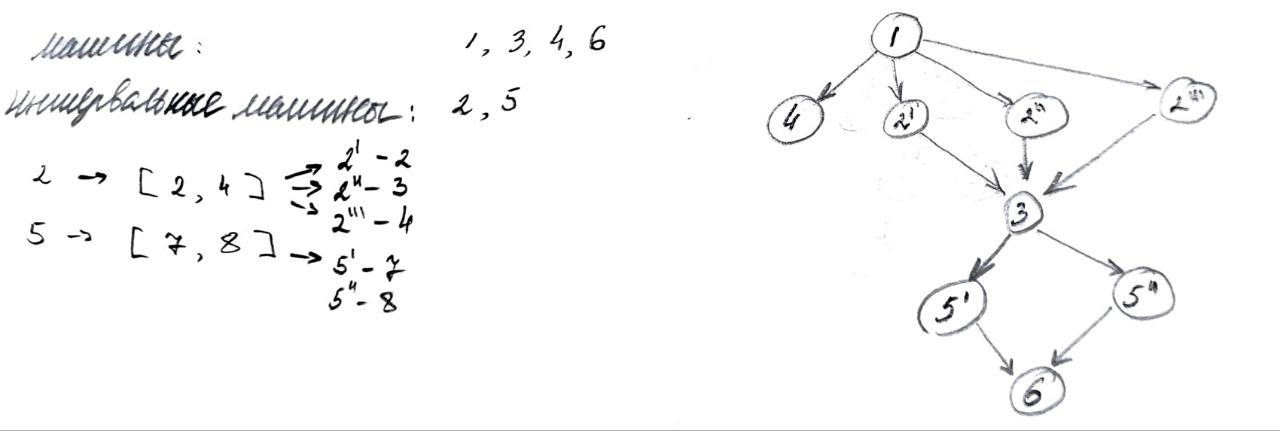
\includegraphics[scale=0.35]{graph}
		\caption{Пример введения фиктивных машин в технологическую карту}
		\label{fig:graph}
	\end{figure}

	\subsection*{Решение №2}
	Также данную задачу можно свести в предыдущей точно так же разбив интервальные машины на фиктивные детерминированные машины и решить несколько задач оптимизации для каждого подмножества всем исходных машин.\\
	
	В рамках предыдущего примера нам нужно решить несколько задач оптимизации со следующими наборами машин:

	\begin{center}
		$\{1, 2', 3, 4, 5', 6\}$\\
		$\{1, 2'', 3, 4, 5', 6\}$\\
		$\{1, 2''', 3, 4, 5', 6\}$\\
		$\{1, 2', 3, 4, 5'', 6\}$\\
		$\{1, 2'', 3, 4, 5'', 6\}$\\
		$\{1, 2''', 3, 4, 5'', 6\}$\\
	\end{center}

	Дальше можно просто выбрать тот набор машин, которые дадут наибольшее значение целевой функции.
\end{document}
